\hypertarget{group__clarke}{}\section{Vector Clarke Transform}
\label{group__clarke}\index{Vector Clarke Transform@{Vector Clarke Transform}}
Collaboration diagram for Vector Clarke Transform\+:
\nopagebreak
\begin{figure}[H]
\begin{center}
\leavevmode
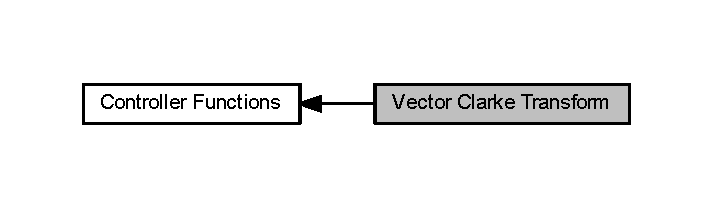
\includegraphics[width=342pt]{group__clarke}
\end{center}
\end{figure}


\subsection{Detailed Description}
Forward Clarke transform converts the instantaneous stator phases into a two-\/coordinate time invariant vector. Generally the Clarke transform uses three-\/phase currents {\ttfamily Ia, Ib and Ic} to calculate currents in the two-\/phase orthogonal stator axis {\ttfamily Ialpha} and {\ttfamily Ibeta}. When {\ttfamily Ialpha} is superposed with {\ttfamily Ia} as shown in the figure below  and {\ttfamily Ia + Ib + Ic = 0}, in this condition {\ttfamily Ialpha} and {\ttfamily Ibeta} can be calculated using only {\ttfamily Ia} and {\ttfamily Ib}.

The function operates on a single sample of data and each call to the function returns the processed output. The library provides separate functions for Q31 and floating-\/point data types. \begin{DoxyParagraph}{Algorithm}
 where {\ttfamily Ia} and {\ttfamily Ib} are the instantaneous stator phases and {\ttfamily p\+Ialpha} and {\ttfamily p\+Ibeta} are the two coordinates of time invariant vector. 
\end{DoxyParagraph}
\begin{DoxyParagraph}{Fixed-\/\+Point Behavior}
Care must be taken when using the Q31 version of the Clarke transform. In particular, the overflow and saturation behavior of the accumulator used must be considered. Refer to the function specific documentation below for usage guidelines. 
\end{DoxyParagraph}
